\documentclass{article}

\usepackage[margin=0.5in]{geometry}
\usepackage{tikz}
\usepackage{tikz-qtree}

\title{Problem Set 1}
\author{Mark Xavier (xaviem01)}

\begin{document}
	
	\maketitle
	
	\begin{enumerate}
		\item Alpha-Beta Pruning - assuming we work left to right and we prune if we decide that a sub-tree is not worth reviewing:
		
		\begin{center}
			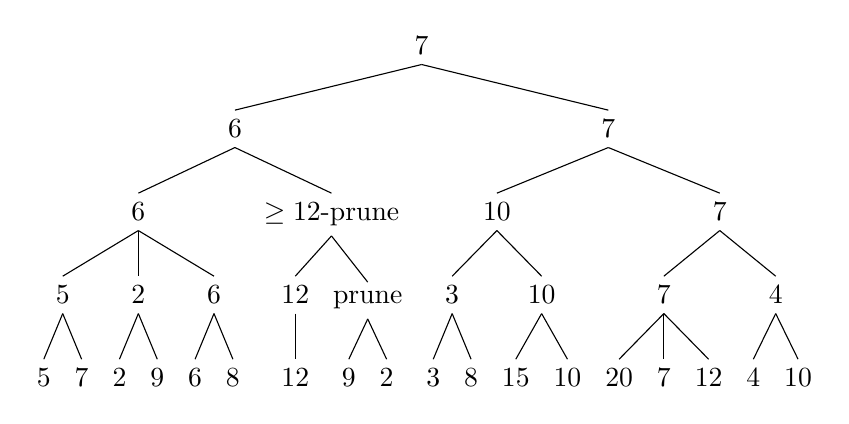
\begin{tikzpicture}
				\Tree[.7 [.6 
				             [.6 
				                 [.5 [.5 ] [.7 ]]  
				                 [.2 [.2 ] [.9 ] ] 
				                 [.6 [.6 ] [.8 ] ]] 
				             [.$\geq12$-prune 
				                 [.12 [.12 ] ] 
				                 [.prune [.9 ] [.2 ] ]]] 
						 [.7
						     [.10 
						         [.3 [.3 ] [.8 ] ] 
						         [.10 [.15 ] [.10 ]]] 
						     [.7
						         [.7 [.20 ] [.7 ] [.12 ]] 
						         [.4 [.4 ] [.10 ]]]] 
					 ]
			\end{tikzpicture}
		\end{center}
	
		I only encountered one area that could be pruned (the node $\geq 12$) - in this case the best move for MAX is to take the right side tree and get a score of 7 as opposed to 6.
	
	\end{enumerate}
	
\end{document}